% 2020 全国Ⅱ卷 理7：多面体的三视图
% 来源 PDF：普通高考/2020/2020全国2理(…).pdf 第 1 页（A3 横排），印面 1121，第 7 题右侧
% 结构：正视图为两块全等长方形（宽 1、高 1.19）上下错开 0.349 拼成，拐角处标 M；
%       侧视图为深 0.853、高 1.539 的矩形，被 y=1.19 与 y=0.349 两条水平线分成三带，
%       中带四角标 E（左上）、F（右上）、G（左下）、H（右下）；
%       俯视图为 2×1 的矩形，被中线分为两个正方形，中线上端标 N。
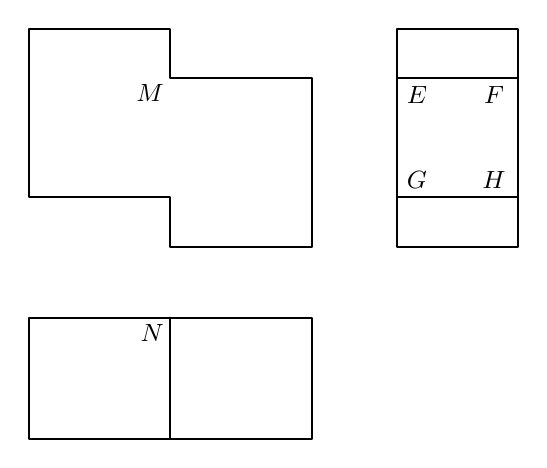
\begin{tikzpicture}[line width=0.7pt, font=\small,
  x=1.8cm, y=1.8cm, line cap=round, line join=round]
  % 尺寸：块宽 1，块高 1.19，块深 0.853，上下错开 0.349
  \def\hh{1.19}
  \def\dd{0.853}
  \def\oo{0.349}
  \def\gt{1.539}

  % 正视图
  \draw (0,\gt) -- (1,\gt) -- (1,\hh) -- (2,\hh) -- (2,0) -- (1,0) -- (1,\oo) -- (0,\oo) -- cycle;
  \node[below left, inner sep=2pt] at (1,\hh) {$M$};

  % 侧视图（左边缘 x=2.6）
  \begin{scope}[shift={(2.6,0)}]
    \draw (0,0) rectangle (\dd,\gt);
    \draw (0,\hh) -- (\dd,\hh);
    \draw (0,\oo) -- (\dd,\oo);
    \node at (0.14,\hh-0.12) {$E$};
    \node at (\dd-0.17,\hh-0.12) {$F$};
    \node at (0.14,\oo+0.12) {$G$};
    \node at (\dd-0.17,\oo+0.12) {$H$};
  \end{scope}

  % 俯视图（上边缘 y=-0.5）
  \begin{scope}[shift={(0,-0.5)}]
    \draw (0,0) rectangle (2,-\dd);
    \draw (1,0) -- (1,-\dd);
    \node[below left, inner sep=2pt] at (1,0) {$N$};
  \end{scope}
\end{tikzpicture}
